\documentclass{standalone}
\usepackage{pgfplots}
\pgfplotsset{compat=1.15}
\usepackage{mathrsfs}
\usetikzlibrary{arrows}
\newcommand{\degre}{\ensuremath{^\circ}}
\pagestyle{empty}

\tikzset{
  pics/handler/.style={perp},
  perp/.pic={                    
    \draw[black,line width=0.4pt](0,-0.05)--(0,.05);
  }
}

\begin{document}
\definecolor{zttcfw}{rgb}{0.5764705882352941,0.23529411764705882,0.9647058823529412}
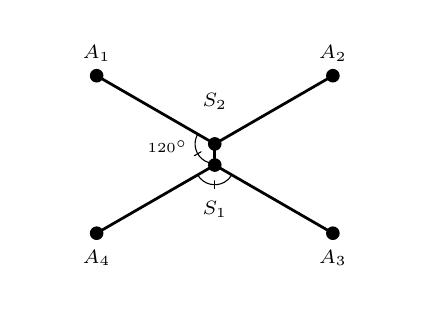
\begin{tikzpicture}[line cap=round,line join=round,>=triangle 45,x=1cm,y=1cm]
    \clip(-0.876026544606624,-0.6034722946554613) rectangle (3.8810217886589404,2.610201760767741);

    % Arcs and angles
    \draw [shift={(1.5,1.134)},line width=0.4pt] (150.00072777015302:0.25) arc (150.00072777015302:270:0.25) pic[pos=.5,sloped]{perp};
    \draw [shift={(1.5,0.8655)},line width=0.4pt] (-150.01505399260216:0.25) arc (-150.01505399260216:-29.984946007397852:0.25) pic[pos=.5,sloped]{perp};

    \begin{scriptsize}
        % Nodes with consistent styling
        \draw(0,2) node[circle,draw, fill=black, scale=0.6] (A1) [label={$A_1$}] {};
        \draw(3,2) node[circle,draw, fill=black, scale=0.6] (A2) [label={$A_2$}] {};
        \draw(3,0) node[circle,draw, fill=black, scale=0.6] (A3) [label={[yshift=-0.6cm]$A_3$}] {};
        \draw(0,0) node[circle,draw, fill=black, scale=0.6] (A4) [label={[yshift=-0.6cm]$A_4$}] {};
        \draw(1.5,0.8655) node[circle,draw, fill=black, scale=0.6] (S1) [label={[yshift=-0.85cm]$S_1$}] {};
        \draw(1.5,1.134) node[circle,draw, fill=black, scale=0.6] (S2) [label={[yshift=0.25cm]$S_2$}] {};

        % Edges
        \foreach \source/\target in {A1/S2, S2/S1, S1/A4, S1/A3, A2/S2} {
                \draw[black, line width=1pt] (\source) -- (\target);
            }

        % Angle label
        \draw[color=black] (0.9,1.1) node {\tiny{$120\textrm{\degre}$}};
    \end{scriptsize}
\end{tikzpicture}
\end{document}